\ifx \twoside \undefined 
\documentclass[12pt,a4paper,oneside,final]{report}
%\documentclass[11pt,a4paper,oneside,draft]{report}
\else
\documentclass[12pt,a4paper,twoside,final,openright]{report}
\fi

% Palatino
\usepackage[T1]{fontenc}
\usepackage[sc]{mathpazo}

% 한글 설정 시작
\usepackage[hangul,nonfrench,finemath]{kotex}
\usepackage[default]{dhucs-interword}
\usehangulfontspec{ut}
\usepackage[hangul]{dhucs-setspace}
\usepackage{dhucs-gremph}

\usepackage{ifpdf}
\ifpdf
  \usepackage[unicode,pdftex,colorlinks=false]{hyperref}
  \input glyphtounicode\pdfgentounicode=1
\else
  \usepackage[unicode,dvipdfm,colorlinks=false]{hyperref}
\fi
% 한글 설정 끝

% Line spacing
\usepackage{setspace}
\doublespacing
%\onehalfspacing

% Header
\pagestyle{headings}

% Bibliography
\usepackage[autostyle=true]{csquotes}
\usepackage[backend=biber,style=ieee,natbib=true,hyperref=true,backref=true,doi=false]{biblatex}
\addbibresource{wjkoh-bs-thesis.bib}
\newcommand{\Kim}{\cite{Kim:2009:SMM:1531326.1531385}} 
\newcommand{\KimKwon}{\cite{Kim:2009:SMM:1531326.1531385,Kwon:2008:GME:1360612.1360679}}
\newcommand{\Igarashi}{\cite{Igarashi:2005:ASM:1073204.1073323}} 
\newcommand{\IgarashiSorkine}{\cite{Igarashi:2005:ASM:1073204.1073323,Sorkine:2004:LSE:1057432.1057456}} 
\newcommand{\Floater}{\cite{Floater200319}} 
\newcommand{\Hormann}{\cite{Hormann:2006:MVC:1183287.1183295}}
\newcommand{\Lipman}{\cite{Lipman:2008:GC:1360612.1360677}}
\newcommand{\Sorkine}{\cite{Sorkine:2004:LSE:1057432.1057456}}
\newcommand{\IgarashiImpl}{\cite{doi:10.1080/2151237X.2009.10129273}}

% Math
\usepackage{amsmath}
\usepackage{amssymb}
%\usepackage{array}
\providecommand{\abs}[1]{\lvert#1\rvert}
\providecommand{\norm}[1]{\lVert#1\rVert}

% Graphics
\usepackage{graphicx}

\newcommand{\thesistitle}{케이지 기반의 대규모 운동 경로 편집\\ (Cage-based Large-scale Motion Path Editing)}

\title{\thesistitle{}}
\author{고우종\\
서울대학교 컴퓨터공학부\\
\href{mailto:wjngkoh@gmail.com}{\texttt{wjngkoh@gmail.com}}
}
\date{\today}
%\keywords{Computer Graphics, Computer Animation,  Data-Driven Animation, Human Motion}

\begin{document}
%% First cover
\begin{titlepage}
\begin{center}
% Upper part of the page
{\LARGE \thesistitle{}}\\[4.0cm]

% Supervisor
{\Large 지도교수 : 이제희}\\[1.5cm]

{\Large 이 논문을 공학학사 학위 논문으로 제출함.}\\[2.5cm]

% Bottom of the page
{\Large \today}\\[1.5cm]
\vfill

% Author
\Large
서울대학교 공과대학\\
컴 퓨 터 공 학 부\\
고 우 종\\[1.0cm]
{\Large 2012년 2월}
\end{center}
\end{titlepage}

\ifx \twoside \undefined 
\else
\newpage
\phantom{placeholder} % doesn't appear on page
\thispagestyle{empty} % if want no header/footer
%\cleardoublepage
\fi

% Another cover
\maketitle

\ifx \twoside \undefined 
\else
\newpage
\phantom{placeholder} % doesn't appear on page
\thispagestyle{empty} % if want no header/footer
%\cleardoublepage
\fi

%\begin{abstract}
%작성중
%\end{abstract}

\tableofcontents

\listoffigures

\chapter{서론}
\begin{figure}[htb]
\centering
%\includegraphics[width=0.8\textwidth]{image.png}
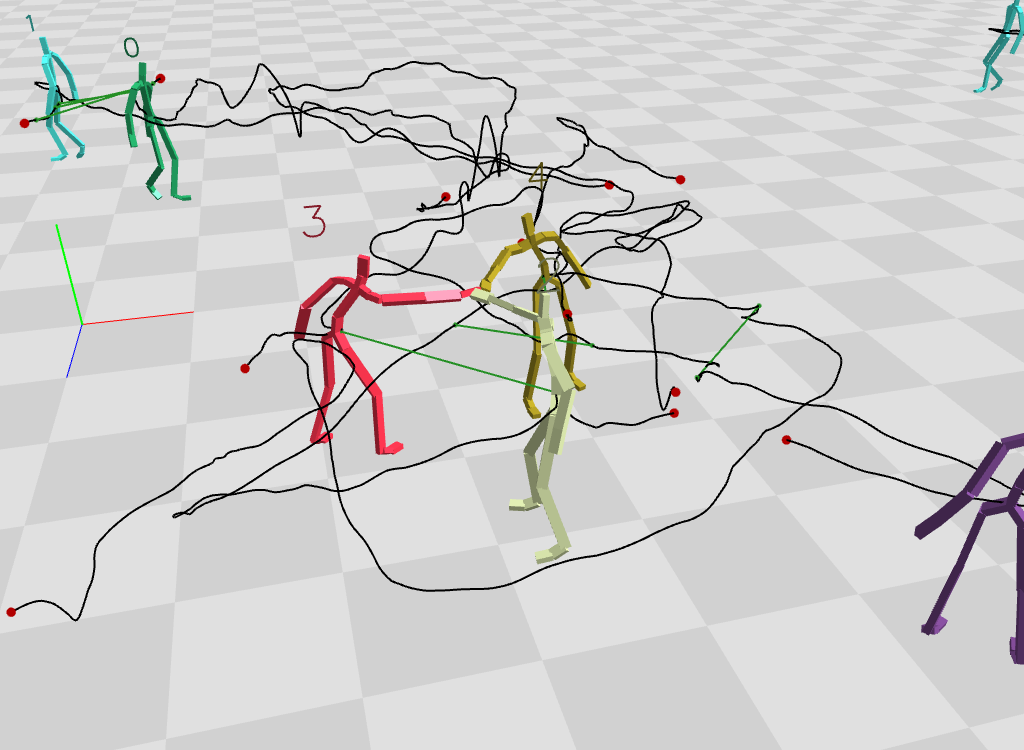
\includegraphics[width=0.9\linewidth]{motion_path_c.png}
\caption{여러 운동 경로로 구성된 장면}
\label{fig:motion_path}
\end{figure}

최근 들어 매우 큰 규모의 군중이 등장하는 장면이 영화나 애니메이션, 비디오 게임
등에 자주 등장하고 있다. 이러한 군중 장면들은 보통
그림~\ref{fig:motion_path}처럼 등장인물들끼리 협동 혹은 적대하는, 여러 개의
상호작용들로 구성되어 있다.  예를 들면 여러 명의 짐꾼이 같은 물건을 동시에
들어서 옮기는 경우나 아니면 여러 명의 병사들이 서로 전투를 하고 있는 장면을 들
수 있다. 이러한 상호작용이 운동 경로 (motion path)에 있어서는 일종의 제약조건
(constraint)으로 작용하는데, 그 이유는 바로 상호작용에 참가하는 각 캐릭터들이
해당 상호작용에 참여하는 다른 캐릭터들과 상대적인 위치, 방향, 타이밍 면에서 잘
조정되어야 하기 때문이다.  본 논문의 목표는 이러한 복잡하게 서로 의존하는 운동
경로들을 상호작용들은 최대한 유지하면서 사용자가 원하는 대로 실시간으로
편집하는 새로운 방법을 개발하는 것이다.

이 문제의 가장 근본적인 어려움은 바로 두 요구사항, 즉 속도와 정확도가 서로
상충하는 역의 관계에 있다는 것이다. 우선, 앞서 언급한 이 제약조건들을 모두
동시에 만족시키기 위해서는 운동 경로 편집 시 매우 정확하고 총체적인 계산이
필요하다.  기존의 방법들은~\KimKwon~운동 경로들의 모든 프레임을 하나의 선형
시스템에 포함시킨 후 이 시스템을 풂으로써 이 문제를 해결하였다. 하지만 이는
질적인 품질을 높이는 대신, 계산 복잡도를 프레임의 총 개수에 의존하게 만듦으로써
기존의 방법을 확장 가능 (scalable)하지 않게 만들었다. 다시 말해 프레임의 총
개수가 증가하게 되면 기존의 방법은 인터랙티브한 편집 속도를 달성하지 못하게
된다.

\begin{figure}[htb]
\centering
%\includegraphics[width=0.8\textwidth]{image.png}
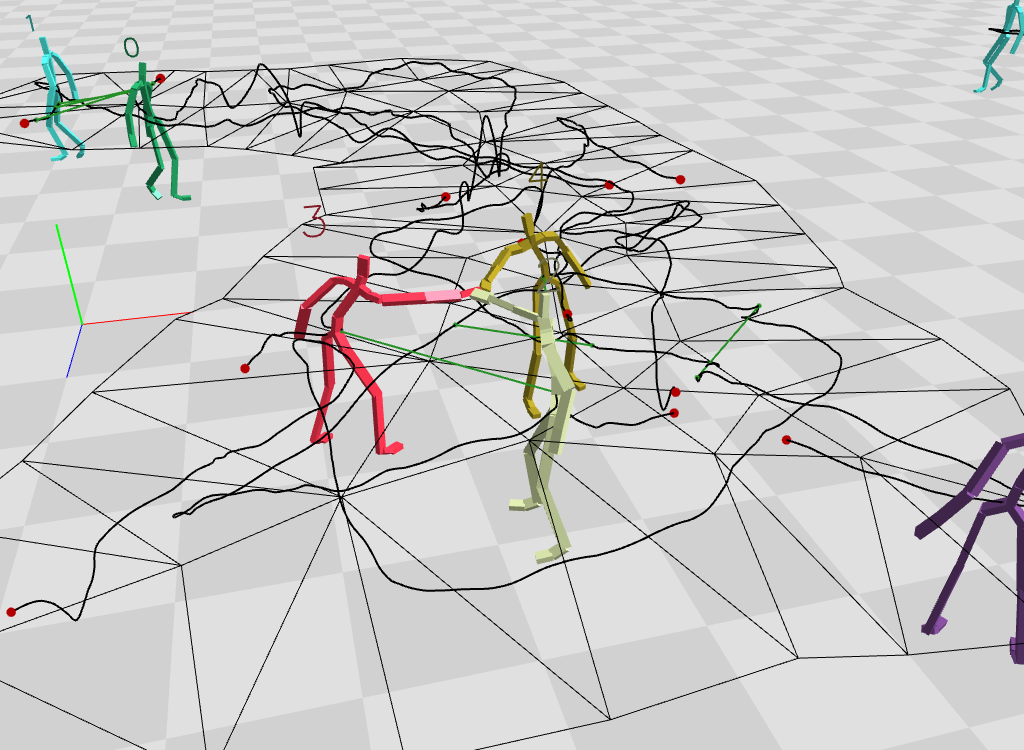
\includegraphics[width=0.9\linewidth]{motion_path_w_mesh_c.png}
\caption{그림~\ref{fig:motion_path}에 2차원 삼각형 메시 (Delaunay)를 씌운 모습}
\label{fig:motion_path_w_mesh}
\end{figure}
 

본 논문의 가장 핵심적인 아이디어는 바로 이처럼 복잡하게 상호 종속적인 운동
경로들의 집합은 서로 분리된 꺾인 곡선들처럼 따로따로 변형되기보다는 마치 2차원
삼각형 메시 (mesh)처럼 같이 변형된다는 관찰에 기반한다. 다시 말해 본 논문에서는
\emph{케이지 기반의 운동 경로 편집}을 이 문제의 해결책으로 제시한다. 간단히
설명하면, 먼저 여러 운동 경로들이 모인 장면에서 경로들을 덮도록 오목 껍데기를
씌우고 이를 작은 삼각형들로 나눠서 그림~\ref{fig:motion_path_w_mesh}처럼 삼각형
메시를 만든다. 그리고 운동 경로들의 모든 프레임의 일반화된 무게중심좌표 (중간값
좌표, 그린 좌표 등) 를 이 삼각형 메시의 외곽 꼭지점들에 대하여 계산한다. 그러고
나면 이 케이지를 가능한 한 잘 휘지 않게 (as-rigid-as-possible) 변형함으로써
그에 맞춰 변형된 운동 경로들을 계산해낼 수 있다. 다시 말해 변형된 프레임들의
좌표는 프레임들의 초기 중간값 좌표 (가중치)와 변형된 케이지의 외곽 꼭지점들
좌표의 가중합 (weighted sum)이다.

%본 논문에서 본 저자가 기여한 바는, 먼저 최대한 덜 휘게 케이지 편집법과
%중간값 좌표의 보간 (interpolation), 매끄러움 (smoothness), 그리고 선형
%정확도 (linear precision) 성질을 이용하여 기존의 계산 과정을 상당부분
%우회할 수 있다는 핵심 아이디어를 낸 것이다. 그리고 또한 실험과정 상에서 

%\section{기존}
%따라서 캐릭터들의 운동 경로 (motion path)들은 이러한 많은 제약조건, 즉 상호
%작용들에 의해 매우 복잡하게 얽혀서 서로 종속성을 강화시킨다.
%
%왜냐하면, 상호작용이 어긋나지 않도록 유지하기 위해서는 각 캐릭터들의 매
%프레임이 위치나 방향, 타이밍 면에서 다른 프레임과 맞도록 매우 미세하게
%조정되어야 하기 때문이다.  더군다나, 이러한 거대한 군중 장면의 사용은 앞으로
%자동화된 생성 방식들이 새로 개발됨에 따라 더욱 널리 사용되어질 것으로 예상된다.
%따라서 이처럼 거대한 군중 장면을 상호작용들은 최대한 그대로 유지하면서
%실시간으로 편집하는 새로운 방법이 애니메이터들에게 필요하게 되었다.

%이 문제를 해결하기 위해, 본 논문에서는 문제를 처음부터 다시 재정의하고 새로운
%접근 방식을 도입했다. 기존의 방식~\cite{Kim:2009:SMM:1531326.1531385}을
%개선시키는 것은 기존 방식의 구조상 내재된 한계에 부딪혔다.  설명하자면, 
%
%이 한계를 극복하기 위해서, 본 저자는 계산 복잡도가 프레임의 총 개수가 아닌,
%고정된 개수의 제어점에만 의존하는 새로운 방법을 고안해냈다. 또한, 더 이상
%애니메이터가 대규모의 군중 장면을 운동 경로 하나하나씩 편집할 수 없으므로,
%조작용 핸들을 새로 정의하였다.
%
%결과적으로, 본 논문에서는 새로운 대규모의 군중 장면을 편집하는 기술을 제시한다.
%이 기술은 애니메이터들에게 원래의 상호작용은 최대한 보존하면서 운동 경로를
%자유자재로 편집할 수 있도록 한다.


\chapter{관련 연구}
기존의 방법~\Kim은 Laplacian curve editing~\Sorkine, 더 정확히 말하면
Laplacian에 비율 조정 (scale adjustment)을 추가한 as-rigid-as-possible curve
editing~\Igarashi을 응용하였다. 이를 이용해 운동 경로를 모든
제약조건들---사용자 정의 제약조건이나 상호작용에 있어서 캐릭터의 위치, 방향,
타이밍 등---을 만족시키면서 부드럽게 변형되도록 했다. 기존의 방법과 달리 새
\emph{케이지 기반의 운동 경로 편집}은 중간값 좌표와 케이지를 도입하여, 운동
경로를 직접적으로 변형하지 않고 대신 케이지를 as-rigid-as-possible mesh
editing~\Igarashi을 사용하여 변형하도록 하고 이로부터 운동 경로를 재구축하도록
하였다.

\section{Mean Value Coordinates} 본 논문에서는 무게중심좌표
(barycentric coordinates)의 일반화 중 하나인 중간값 좌표 (mean value
coordinates)를 사용하였다. 이 좌표는 조화함수를 위한 중간값 정리에서 착안하여
만들어진 좌표로서, 다각형의 꼭지점들에 매겨진 값들로부터 중간값들을 보간하는데
유용하다~\Floater.

무게중심좌표는 볼록다각형에는 적용할 수 있으나 볼록하지 않은 다각형에 대해서는
일반적으로 적용할 수 없다. 반면에 중간값 좌표는 모서리끼리 스스로 교차하지
않는, 임의의 평면다각형에 대해서도 잘 정의된다~\Hormann. 운동 경로들을 정교하게
덮기 위해서는 오목 껍데기 (concave hull)를 사용해야 하므로 본 논문에는
무게중심좌표보다 중간값 좌표가 더 적합하다.

중간값 좌표의 정의를 간단히 설명하면 다음과 같다. 2차원 상의 점 $x \in
\mathbb{R}^2$ 와 순환적으로 정의된 단순 다각형 (simple polygon) $[v_0, v_1,
..., v_k, v_{k+1} = v_0]$이 있다 하자. 그리고 각 $\alpha_i$를 그 다각형의 각
$\angle v_{i+1},x,v_{i}$라 하자.

\begin{align}
\lambda_i = \frac{w_i}{\sum_{j=1}^{k}w_j}, \quad w_i =
2\frac{\tan(\alpha_{i-1}/2) + \tan(\alpha_{i}/2)}{\norm{x - v_i}}
\end{align}

그러면 가중치 $(\lambda_0, ..., \lambda_k)$가 바로 $x$의 $v_0, ...  , v_k$에
대한 중간값 좌표가 된다.

\section{Green Coordinates}
그린 좌표 (Green coordinates) 역시 오목다각형에도 적용할 수 있는
무게중심좌표의 일반화 중 하나이다. 계산 과정은 조금 더 복잡하지만, 그린 좌표는
2차원에서 순수 등각사상 (pure conformal mapping)이므로 원래 운동 경로의 형태를
중간값 좌표보다 더 잘 보존하는 특성을 가지고 있다~\Lipman.

\chapter{케이지 기반의 운동 경로 편집}
\section{개괄}
\emph{케이지 기반의 운동 경로 편집}을 대략적으로 설명하면 다음과 같이 서술할 수 있다.
먼저, 운동 경로들을 덮는 최소한의 볼록 혹은 오목 껍데기를 만들고 이를
삼각형으로 나누어서 2차원 삼각형 메시를 구성한다. 그리고 as-rigid-as-possible
triangle mesh editing~\Igarashi을 사용하여 이 삼각형 메시를 사용자가 원하는
대로 변형시킨다. 사용자는 이 삼각형 메시의 어떤 꼭지점이라도 마음대로 움직이고
고정시킬 수 있다. 그러고 나면 이 변형된 삼각형 메시, 정확히는 메시의 외곽
꼭지점들로부터 변형된 운동 경로들을 계산해낼 수 있다.

더 자세히 설명하면, 운동 경로들의 모든 프레임은 이 삼각형 메시의 외곽
꼭지점들과 그 꼭지점들에 대한 중간값 좌표로 표현할 수 있다. 따라서 케이지의
역할을 하는 이 삼각형 메시가 원래 형태를 최대한 유지하려고 노력하면서
변형된다면, 중간값 좌표의 보간 (interpolation), 매끄러움 (smoothness), 그리고
선형 정확도 (linear precision) 성질 덕분에 중간값 좌표로 표현된 운동 경로들
역시 부드럽게 변형된다. 새 방법은 기존의 방법과는 달리 모든 프레임이 포함된
선형 시스템을 풀 필요가 사라지므로 매우 빠른 속도로 계산을 완료할 수 있다.

\section{알고리즘}
앞서 언급했듯이 기존의 편집 방법~\Kim은 as-rigid-as-possible \emph{curve}
editing~\Igarashi에 사용자 정의 제약조건을 추가한 다음 운동 경로에 적용함으로써
원하는 결과를 얻어내었다.  본 논문 역시 비슷하게 as-rigid-as-possible
\emph{triangle mesh} editing~\Igarashi에 사용자 정의 제약조건을 추가한 다음
이를 운동 경로가 아닌 케이지에 적용하였다. 그리고 이 변형된 케이지에서 중간값
좌표를 통해 운동 경로를 재구축함으로써 원하는 결과를 얻었다.

이 사용자 정의 제약조건을 추가하는 방법에 대한 실마리는 Takeo Igarashi의 후속
논문에서 발견할 수 있었다. 이 후속 논문의 5절, \emph{Allowing Handles on
Arbitrary Positions in the
Mesh}~\cite[p.26]{doi:10.1080/2151237X.2009.10129273} 에 기술된 대로 구현하면
삼각형 메시의 꼭지점들뿐만 아니라 메시 안의 임의의 점들도 핸들로 잡고 고정시킬
수 있다.  따라서 이를 이용하여 운동 경로의 위치 제약조건을 구현할 수 있었다.
그리고 사용자 정의 제약조건 역시 사용자가 메시의 꼭지점 뿐만아니라 임의의 점을
잡고 변형할 수도 있게 되었다.

따라서 첫 번째 과정인, 제약조건들을 만족하면서 as-rigid-as-possible하게 삼각형
메시를 마음대로 변형하는 것은 상대적으로 수월하게 구현할 수 있었다. 그리고 두
번째 과정인, 변형된 메시에서 변형된 운동 경로들을 재구축하는 것은 프레임들의
초기 중간값 좌표와 변형된 메시의 외곽 꼭지점 좌표들의 단순한 선형 조합 (linear
combination)이므로 벡터와 벡터의 곱으로 간단하게 구할 수 있었다.

\chapter{결과}
계산 소요시간 측정 실험에 사용된 환경은 다음과 같다. 테스트 머신의 CPU는 Intel
Core2 Quad 2.40GHz였으며 RAM은 4GB였다. 운영체제는 Microsoft Windows 7
Enterprise (64-bit)를 사용하였고 실험 프로그램은 C++로 작성하여 Microsoft
Visual Studio 2010 Professional로 컴파일하였다.

실험에 사용된 데이터는 그림~\ref{fig:motion_path}과
그림~\ref{fig:before_deform}에서 볼 수 있는, 모션 캡처된 운동 경로 6개로 구성한
하나의 장면이다. 모션 캡처 데이터는 16개의 카메라를 쓰는 Vicon 모션 캡처
시스템을 사용하여 120 프레임/초의 속도로 캡처하였고 30 프레임/초로
서브샘플링하였다.

\begin{table}[ht]
\centering
\begin{tabular}{c|c}
\hline
항목 & 개수 \\
\hline
총 운동 경로 & 6 \\
총 프레임 & 3809 \\
메시의 삼각형 & 110 \\
메시의 꼭지점 & 81 \\
\hline
\end{tabular}
\caption{실험에 사용된 데이터}
\label{table:data}
\end{table}

\begin{figure}[p]
\centering
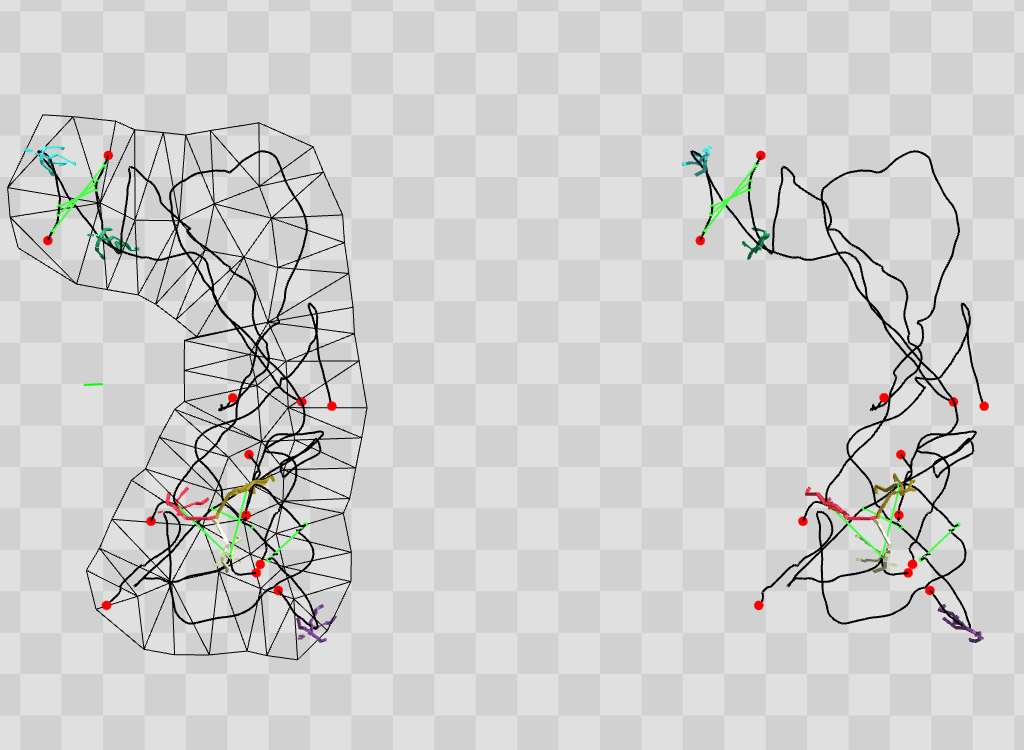
\includegraphics[width=0.9\linewidth]{before_deform_c.png}
\caption{변형 전}
\label{fig:before_deform}
\end{figure}

\begin{figure}[p]
\centering
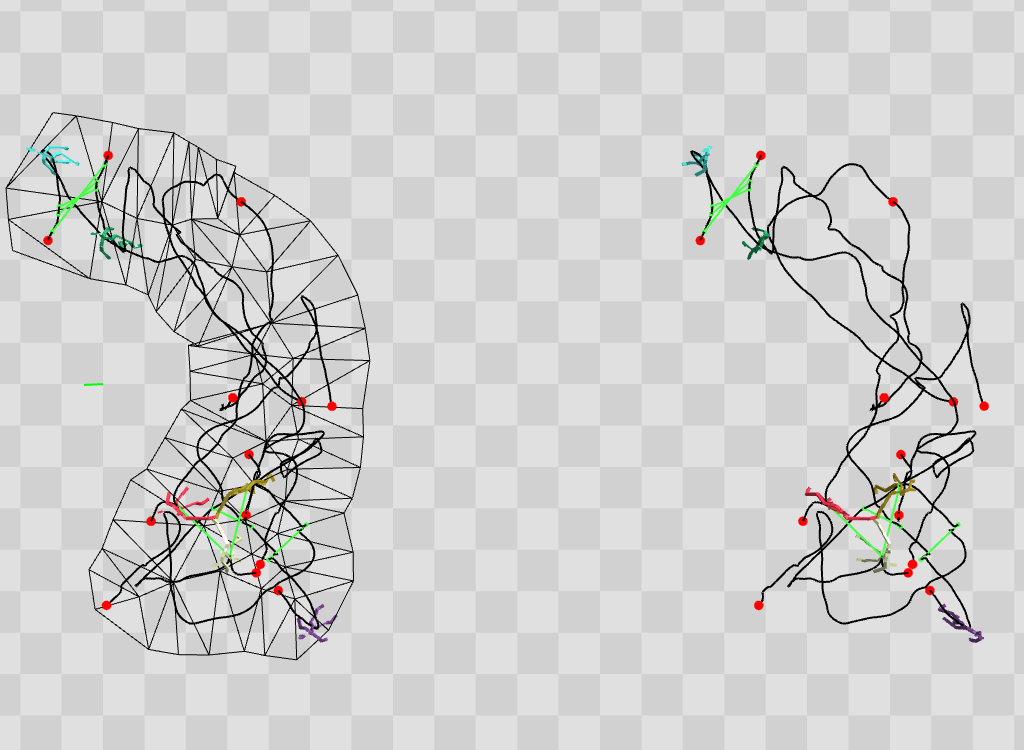
\includegraphics[width=0.9\linewidth]{after_deform_c.png}
\caption{변형 후 (좌) 본 논문의 방법 (우) 기존 Laplacian editing}
\label{fig:after_deform}
\end{figure}

\begin{table}[ht]
\centering
\begin{tabular}{r*{2}{r}c}
\hline
 & \multicolumn{2}{c}{계산 소요시간 (ms)} & \\
\cline{2-3}
회차 & 기존 방법 & 새로운 방법 & 속도 향상 (배) \\
\hline
1 & 1437 & 14 & 102.64 \\
2 & 1469 & 14 & 104.93 \\
3 & 1446 & 14 & 103.29 \\
4 & 1391 & 13 & 107.00 \\
5 & 1440 & 13 & 110.77 \\
6 & 1444 & 13 & 111.08 \\
7 & 1386 & 13 & 106.62 \\
8 & 1444 & 13 & 111.08 \\
9 & 1394 & 13 & 107.23 \\
10 & 1442 & 13 & 110.92 \\
\hline
평균 & 1429.3 & 13.3 & 107.55 \\
\hline
\end{tabular}
\caption{계산 소요시간 측정 결과}
\label{table:result}
\end{table}

측정해본 결과, 표~\ref{table:result}에서 볼 수 있듯이 기존 방법과 비교해 \emph{약
107.55배}의 속도 향상을 확인할 수 있었다.

\chapter{결론}
결과적으로 이 새로운 \emph{케이지 기반의 운동 경로 편집}을 통해 계산 복잡도를
매우 큰 폭으로 낮출 수 있었고 편집 과정을 확장 가능 (scalable)하게 만들 수
있었다. 그 이유는 이 새로운 방법의 계산 복잡도는 케이지라는 중간 매개체가
도입됨으로써 운동 경로들의 프레임 총 개수에 의존적이지 않고 케이지의 꼭지점 총
개수에 의존적이게 되었기 때문이다. 또한, 케이지의 꼭지점들을 새로운 조작
핸들로서 제시하여 애니메이터들이 거대한 군중 장면을 쉽게 편집할 수 있도록
하였다.

%future work
하지만 본 논문의 방법은 작은 변형 (small deformation)의 경우에는 상대적
제약조건 (relative constraint)---상호작용시 캐릭터 간의 거리, 방향 그리고
타이밍 등---이 잘 맞지만 큰 변형 (large deformation)에서는 어긋날 수 있다.
따라서 차후 과제로는 상대적 제약조건을 확실하게 보장해주도록 개선하는 것을 들
수 있다. 다시 말해 2차원 삼각형 메시 변형시 삼각형의 형태와 사용자 정의
제약조건만 최대한 유지하도록 하는 것이 아니라 이 상대적 제약조건도 최대한
지키도록 만드는 것이 앞으로 남은 과제이다.

\printbibliography
\end{document}
